\section{Chinese Grand Prix}

\subsection{Circuit Analysis}

\textbf{Circuit Name:} Shanghai International Circuit (Shanghai, China) \\
\textbf{Length:} 5.451 km - \textbf{Laps:} 56 - \textbf{Total Distance:} 305.066 km

\begin{figure}[H]
    \centering
    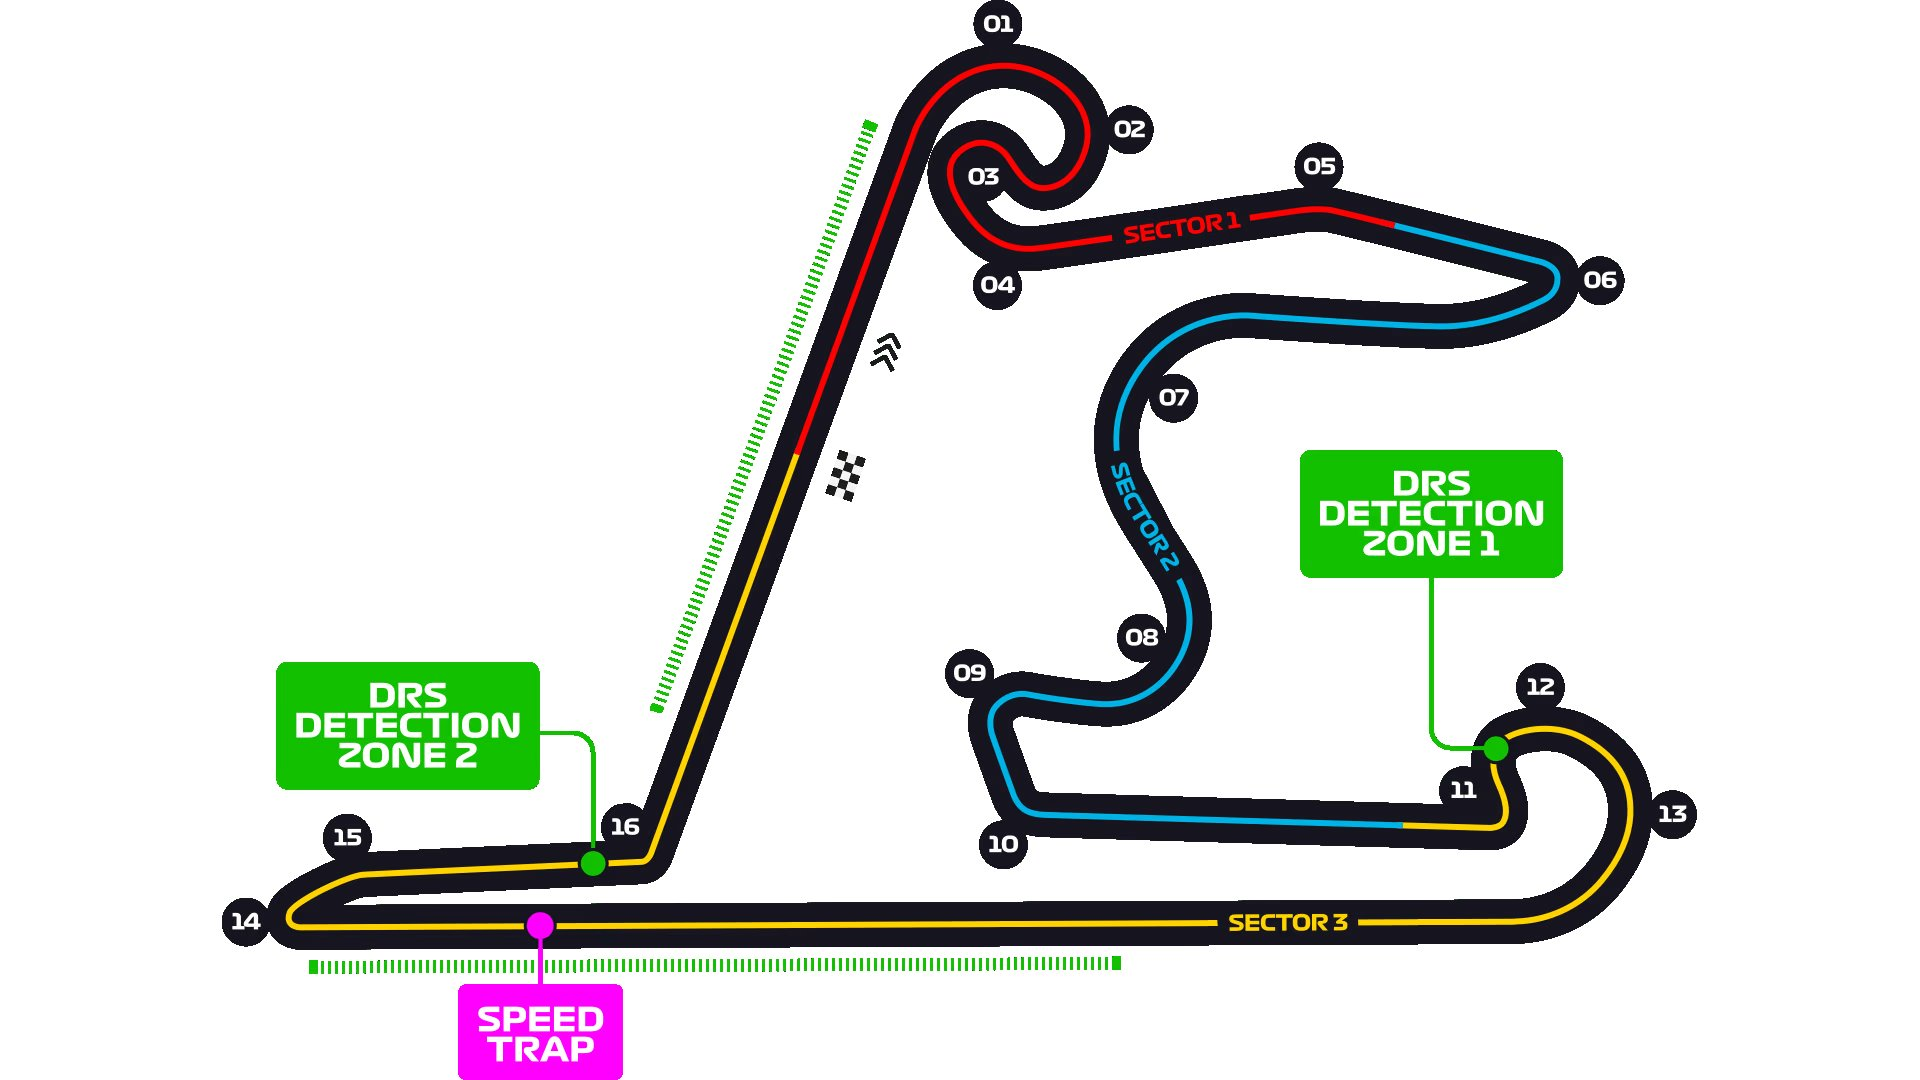
\includegraphics[width=0.75\linewidth]{images/5.China_Circuit.jpg}
\end{figure}

\begin{itemize}
    \item \textbf{Lap Record} : 1:31.095 (2018, Sebastian Vettel – Ferrari).

    \item \textbf{Number of Corners \& Key Features} : 16 turns (9 right, 7 left). \\
    Famous opening complex (Turns 1–2) with a tightening radius, long back straight (1.2 km) leading to heavy braking at Turn 14. \\
    Mix of high-speed esses (Turns 7–8) and slow technical corners (Turn 6, Turn 11).

    \item \textbf{Braking Zones \& Traction} : Major braking at Turn 14 (down from ~330 km/h to 70 km/h). \\
    Traction is critical exiting Turns 6, 13 and 14 due to long acceleration phases.

    \item \textbf{DRS \& Overtaking} : Two DRS zones (start/finish straight, long back straight). \\
    Turn 14 is the prime overtaking zone, Turn 6 also offers chances.

    \item \textbf{Tyre Degradation \& Strategy} : Front-left tyre wear is a known issue due to long right-handers. \\
    Most teams targeted two-stop strategies, but one-stop possible with tyre management.

    \item \textbf{Weather \& Environment} : Cool spring conditions, track temp lower than Middle East races. \\
    Wind and smog sometimes affect visibility and downforce balance.
\end{itemize}

\textbf{Strategic Summary :}  
Shanghai demands strong aerodynamic efficiency for the high-speed esses and mechanical grip for the slow hairpins. The long back straight rewards power units and top speed, while tyre wear (front-left) requires careful management. Strategy flexibility (1–2 stops) is crucial depending on tyre degradation.

\subsection{Race Analysis}

\textbf{Date:} Sprint : 20 April 2024 - 11:00 local time\\
Race : 21 April 2024 — 15:00 local time 

\begin{itemize}
    \item \textbf{Sprint Qualifying:} \textbf{Pole Position:} Lando Norris (McLaren) - 1:57.940.\\
    Grid : Hamilton 2nd, Alonso 3rd, Verstappen 4th.

    \item \textbf{Sprint Summary} : \textbf{Winner:} Max Verstappen (Red Bull). \\
    \textbf{Podium}: 1. Verstappen - 2. Hamilton - 3. Pérez. \\
    Norris, who started from pole, went wide Lap 1 and fell to P6.\\
    Alonso (10s penalty) retired after contact with Sainz.

    \item \textbf{Qualifying Summary} : \textbf{Pole Position:} Max Verstappen (Red Bull) - 1:33.660. \\
    Grid: Pérez 2nd, Alonso 3rd, Norris 4th.\\

    \item \textbf{Race Summary} : \textbf{Winner:} Max Verstappen (Red Bull) — dominant pace, controlled from the front. \\
    \textbf{Podium:} 1. Verstappen - 2. Norris - 3. Pérez . \\
    Alonso, after starting P3, faded with tyre wear and ended P7 but took fastest lap.\\
    \textbf{Technical issues:} Bottas (engine - Virtual Safety Car lap 20).\\
    \textbf{Notable incidents:} Ricciardo crashed because of Stroll (10s penalty) + Tsunoda crashed because of Magnusssen (10s penalty) (Safety Car lap 26).

    \item \textbf{Strategies} : Most drivers adopted a two-stop race due to heavy front-left degradation. \\
    - Red Bull ran Soft–Hard–Medium, Verstappen extending his middle stint to stay in control even after the Safety Car. \\
    - Norris benefited from a perfectly timed stop under VSC on lap 20, which allowed him to jump Alonso and challenge Pérez. \\
    - Ferrari committed to a standard two-stop plan but suffered graining on the Mediums, which limited their race pace. \\
    - Mercedes split approaches: Russell on Soft–Medium–Hard, while Hamilton started from P18 with a more aggressive Soft–Medium–Medium that helped him recover to P9. \\
    - Alonso attempted a three-stop strategy to mitigate tyre wear. Although it cost him track position, he secured the fastest lap in the closing stages. \\

    \item \textbf{Performance Trends} : \textbf{Red Bull} — Verstappen dominant (led 51/56 laps), Pérez solid P3. Car excelled in traction + straights.\\
    \textbf{McLaren} — Norris capitalised on SC timing, excellent straight-line speed, secured P2 and Driver of the Day.\\
    \textbf{Ferrari} — Leclerc P4, Sainz P5. Tyre degradation (front-left graining) limited their challenge.\\
    \textbf{Mercedes} — Russell P6 consistent, Hamilton recovered from P18 to P9.

    \item \textbf{Championship Impact} : \textbf{Drivers:} Verstappen 110 points, Pérez 85, Leclerc 76.\\
    \textbf{Constructors:} Red Bull 195, Ferrari 151, McLaren 96, Mercedes 52.
\end{itemize}

\textbf{Key Takeaway :}  
Red Bull confirmed their superiority on a mixed circuit layout, Verstappen flawless from pole. McLaren proved highly competitive on power-sensitive tracks, while Ferrari’s tyre weakness cost them.

\subsection{Link \& Takeaway}

\begin{itemize}
    \item Shanghai’s long straights and heavy braking zones rewarded Red Bull’s traction and straight-line speed.
    \item Norris and McLaren capitalised on their efficiency to secure P2, confirming progress on power tracks.
    \item Ferrari’s tyre degradation issues (front-left wear) matched circuit expectations and limited their challenge.
    \item Safety Car and penalties affected midfield but not the Verstappen-led top order, showing how dominant Red Bull remained.
    \item Alonso’s fastest lap underlined Aston Martin’s potential on fresh tyres but highlighted lack of long-run race pace.
\end{itemize}
